%χαρακτηριστικά κειμένου
\documentclass[10pt, a4paper]{article}
% Χρήση γλωσσών
\usepackage[utf8]{inputenc}
\usepackage[draft=false, colorlinks=true, allcolors = black, urlcolor=blue]{hyperref} %set url colors
\usepackage{graphicx} % for better use of images
\graphicspath{{figures}} %Setting the graphicspath containing images/figures

\usepackage{minted} % used for embedding code in the report

\usepackage{amsmath} % used for multiline math expressions
\usepackage{tcolorbox} % used for R code formatting
\tcbuselibrary{minted,skins}

\usepackage{placeins} % used to properly place figures in their subsections and not next ones

\usepackage{url} % used for using urls in the references section

% FIRST PAGE OF DOCUMENT
% NTUA logo on top

\pagenumbering{gobble} %remove page numbering
\begin{figure}
    \centering
    
\includegraphics[width=3cm]{/NTUA_logo_transparent.png}
\end{figure}

\title{
National Technical University of Athens \\
MSc - Data Science and Machine Learning \\\ \\\
\textbf{Geospatial Big Data Analytics} \\
\vspace*{1cm}
Lab 2\\
Geospatial Services and Web Applications
\vspace*{4cm}}

\author{Vasileios Depastas \\ MSc student \\ \\ A.M: 03400131 \\
\href{mailto:vasileiosdepastas@mail.ntua.gr}{vasileiosdepastas@mail.ntua.gr} 
}
\date{\vspace*{4cm}May 2022}


\begin{document}

\maketitle %create the first page that contains the title and all other elements

\newpage %start of a new page

\thispagestyle{empty}
\tableofcontents
    
\listoffigures
    
\listoftables
    
\clearpage
\newpage
\pagenumbering{arabic} %reenable page numbering

\section{Introduction}
In this exercise, we experiment with some of the most widely used libraries and APIs for importing, processing and visualizing geospatial data. During the implementation, we also make use of relevant web services-applications and the standards of the Open Geospatial Consortium (OGC). \\

Some of the libraries that were used are the following ones:\\

\begin{tabular}{ | p{1.5cm} | p{7cm}| } 
  \hline
  Library & Usage \\
  \hline
  OWSLib & Python package for client programming with OGC web service interface standards.\\
  \hline
  rasterio & Python module for raster image processing used for reading and writing several raster formats. \\ 
  \hline
  geopandas & Extension of Python's pandas library's datatypes to allow spatial operation on geometric type. Depends on shapely library for geometric operations, fiona for file accessing and matplotlib for plotting.\\ 
  \hline
  fiona & Python library for reading and writing geographic vector data files. \\ 
  \hline
  folium & Python's library used for visualizing geospatial data. A wrapper of leaflet.js javascript library for interactive maps plotting. \\ 
  \hline
  leafmap & Python package for interactive mapping and geospatial analysis in a Jupyter notebook environment.\\
  \hline
\end{tabular}


\section{Question 2}
Here, we present raster image data by visualizing different bands and spectral indexes as well as their variation over time.  
\subsection{ Question 2.1}
First of all, we download Sentinel-2 images of the broader \textbf{Kastoria region} (ROI) in northern Greece from \href{https://pithos.okeanos.grnet.gr/public/fBSNLJeNxerluMj2MVDqF}{here}. A pdf file explaining the dataset accompanies the image series. According to that, the dataset contains two \emph{.tif} large files:

\begin{enumerate}
  \item \emph{Kastoria.tif}: 24 raster images spanning from 25-01-2016 until 30-12-2016 (corresponding doy range: 25 - 365) with 10 bands per image. This results in a spectro-temporal cube of dimension 240 x 2017 x 2281.
  \item \emph{Kast\_RefData\_26Classes.tif}:  image with 26 class codes for different land usages classification.
\end{enumerate}

To load the data, we make use of the rasterio library. From the image collection of \emph{Kastoria.tif}, we then select the first image's blue band according to the tiff's pdf documentation downloaded. We can then use either matplotlib or rasterio to plot the image's band. However, using rasterio's plot.show() function allows us to maintain proper geo-referenced labeling for the two axes. Therefore, we will prefer this plot type moving forward.

\begin{figure}[h]
    \centering
    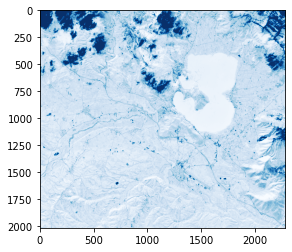
\includegraphics[width=7cm]{figures/q2_1_matplotlib_image1_blue_band.png}
    \caption{Kastoria region - image: 1, band: blue, matplotlib}
    \label{fig:Kastoria region - image: 1, band: blue, matplotlib}
\end{figure}
\FloatBarrier %fix position of image to its own subsection, not the next

\begin{figure}[h]
    \centering
    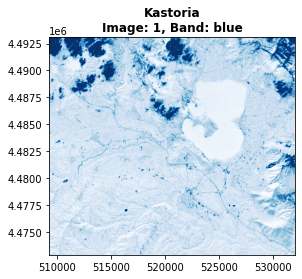
\includegraphics[width=7cm]{figures/q2_1_rasterio_image1_blue_band.png}
    \caption{Kastoria region - image: 1, band: blue, rasterio}
    \label{fig:Kastoria region - image: 1, band: blue, rasterio}
\end{figure}
\FloatBarrier %fix position of image to its own subsection, not the next

Then, for this first image of the dataset, we plot alongside each other the three bands, Red, Green and Blue.

\begin{figure}[h]
    \centering
    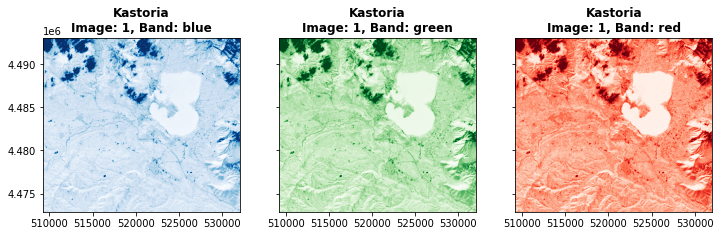
\includegraphics[width=13cm]{figures/q2_1_rasterio_image1_rgb_bands.png}
    \caption{Kastoria region - image: 1, bands: red, green, blue}
    \label{fig:Kastoria region - image: 1, bands: red, green, blue}
\end{figure}
\FloatBarrier %fix position of image to its own subsection, not the next

We also plot the RGB image of the dataset's first image for the Kastoria region by combining the three bands, Red, Green and Blue.

\begin{figure}[h]
    \centering
    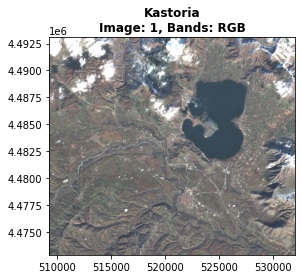
\includegraphics[width=7cm]{figures/q2_1_rasterio_image1_rgb_image.png}
    \caption{Kastoria region - image: 1, RGB}
    \label{fig:Kastoria region - image: 1, RGB}
\end{figure}
\FloatBarrier %fix position of image to its own subsection, not the next

Moving forward, we calculate the NDVI index band for the first image of the image collection dataset using the near infrared (NIR) and RED bands as $ NDVI = \frac{NIR-RED}{NIR+RED}$. Using this band, we can then create a histogram of the values for the ndvi band for all the image's pixels as well as plot the image of the ndvi band in  red-yellow-green color map

\begin{figure}[h]
    \centering
    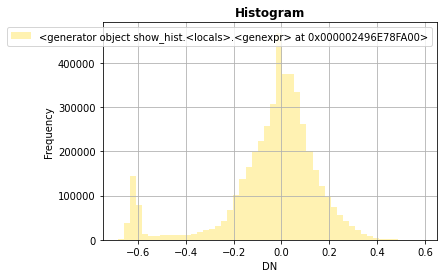
\includegraphics[width=8cm]{figures/q2_1_image1_ndvi_histogram.png}
    \caption{Kastoria region - image: 1, ndvi histogram}
    \label{fig:Kastoria region - image: 1, ndvi histogram}
\end{figure}
\FloatBarrier %fix position of image to its own subsection, not the next

\begin{figure}[h]
    \centering
    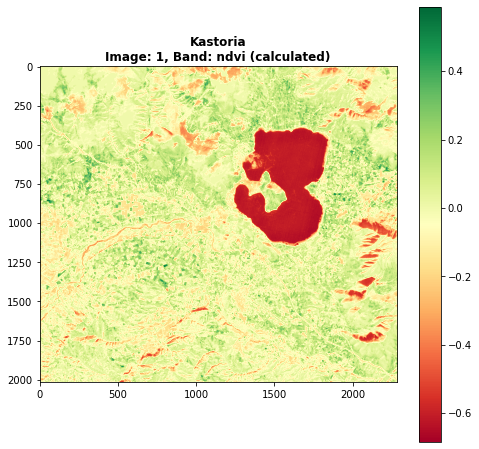
\includegraphics[width=8cm]{figures/q2_1_image1_ndvi_map.png}
    \caption{Kastoria region - image: 1, ndvi}
    \label{fig:Kastoria region - image: 1, ndvi}
\end{figure}
\FloatBarrier %fix position of image to its own subsection, not the next

In general, NDVI values range from -1.0 to 1.0, with negative values indicating clouds and water, positive values near zero indicating bare soil, and higher positive values of NDVI ranging from sparse vegetation (0.1 - 0.5) to dense green vegetation (0.6 and above). Given that the first image is taken on 25-01-2016, and hence during winter time, the vegetation observed is mostly sparse rather than dense.

\subsection{Question 2.2}
Now, we select a polygon as a region of interest (ROI) within the broader Kastoria region for which we will retrieve raster, vector and timeseries data using different data sources. 
Towards this purpose, we use geojson.io to draw a polygon region of interest (ROI) in Kastoria and download the shapefile related to that in order to clip it afterwards from the images of the dataset and concentrate subsequent steps on that ROI solely. A shape files stores both the geometric location and attribute information of geographic features like lines, points or polygons. Clipping an image is also called masking (of a raster file by a shape file). To read a shapefile we utilize the \emph{geopandas} library.

Loading the shapefile with geopandas, we were able to identify its coordinate reference system (crs) as EPSG:4326, which is different to the one of the Kastoria raster images dataset, EPSG:32634. Therefore, a transform was performed to the dataset. 

\begin{figure}[h]
    \centering
    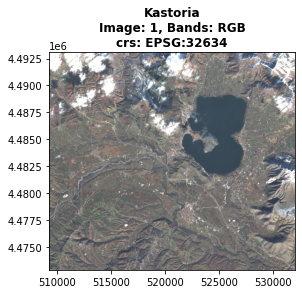
\includegraphics[width=7cm]{figures/q2_1_rasterio_image1_rgb_image_old_crs.png}
    \caption{Kastoria region - image: 1, RGB, EPSG:32634}
    \label{fig:Kastoria region - image: 1, RGB, EPSG:32634}
\end{figure}
\FloatBarrier %fix position of image to its own subsection, not the next

\begin{figure}[h]
    \centering
    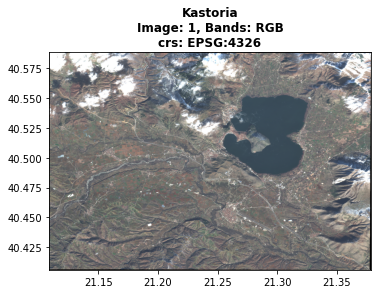
\includegraphics[height=7cm]{figures/q2_1_rasterio_image1_rgb_image_new_crs.png}
    \caption{Kastoria region - image: 1, RGB, EPSG:4326}
    \label{fig:Kastoria region - image: 1, RGB, EPSG:4326}
\end{figure}
\FloatBarrier %fix position of image to its own subsection, not the next

Once the crs transform has been completed, we can see that the two axes values have changed. The image can be now clipped with the selected polygon. First, we open the shapefile with fiona this time and then mask the raster dataset with the vector data using rasterio's mask function. We end up with 240 images with size $width x height = 534 x 389 $ with EPSG:4326 crs. In the next image, we can see in blue the selected polygon ROI in Kastoria. Any subsequent analysis and steps will concern this ROI.

\begin{figure}[h]
    \centering
    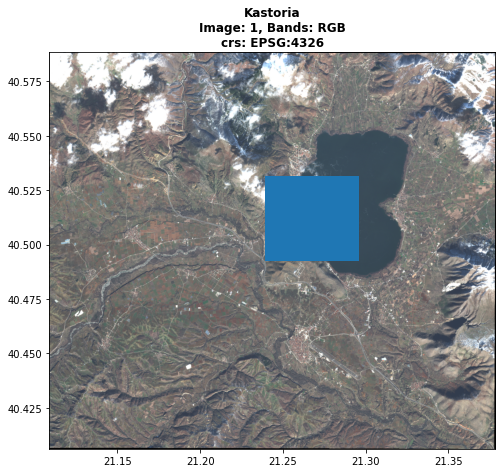
\includegraphics[width=6cm]{figures/q2_2_mask_ROI.png}
    \caption{Kastoria ROI mask}
    \label{fig:Kastoria ROI mask}
\end{figure}
\FloatBarrier %fix position of image to its own subsection, not the next

We can see that the clipped area selected (ROI) is a rectangular that contains both water and land areas in Kastoria in order to spot the differences in different types of land usage in subsequent analysis.

Next, we plot the first image (first date) of the clipped dataset in RGB.

\begin{figure}[h]
    \centering
    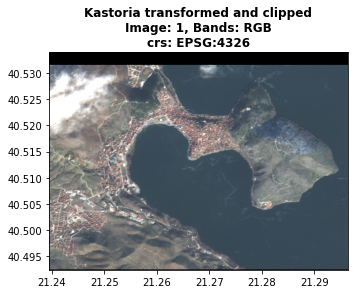
\includegraphics[width=6cm]{figures/q2_2_ROI_clipped_RGB.png}
    \caption{Kastoria ROI, Image: 1, RGB}
    \label{fig:Kastoria ROI, Image: 1, RGB}
\end{figure}
\FloatBarrier %fix position of image to its own subsection, not the next

\subsection{Question 2.3}
Upon transforming the crs of the dataset and clipping all 24 images of the dataset to the selected polygon ROI, we now move on to visualize the NDVI index for each available date as well as to calculate the average NDVI index value across all pixels in the ROI.

\begin{figure}[h]
    \centering
    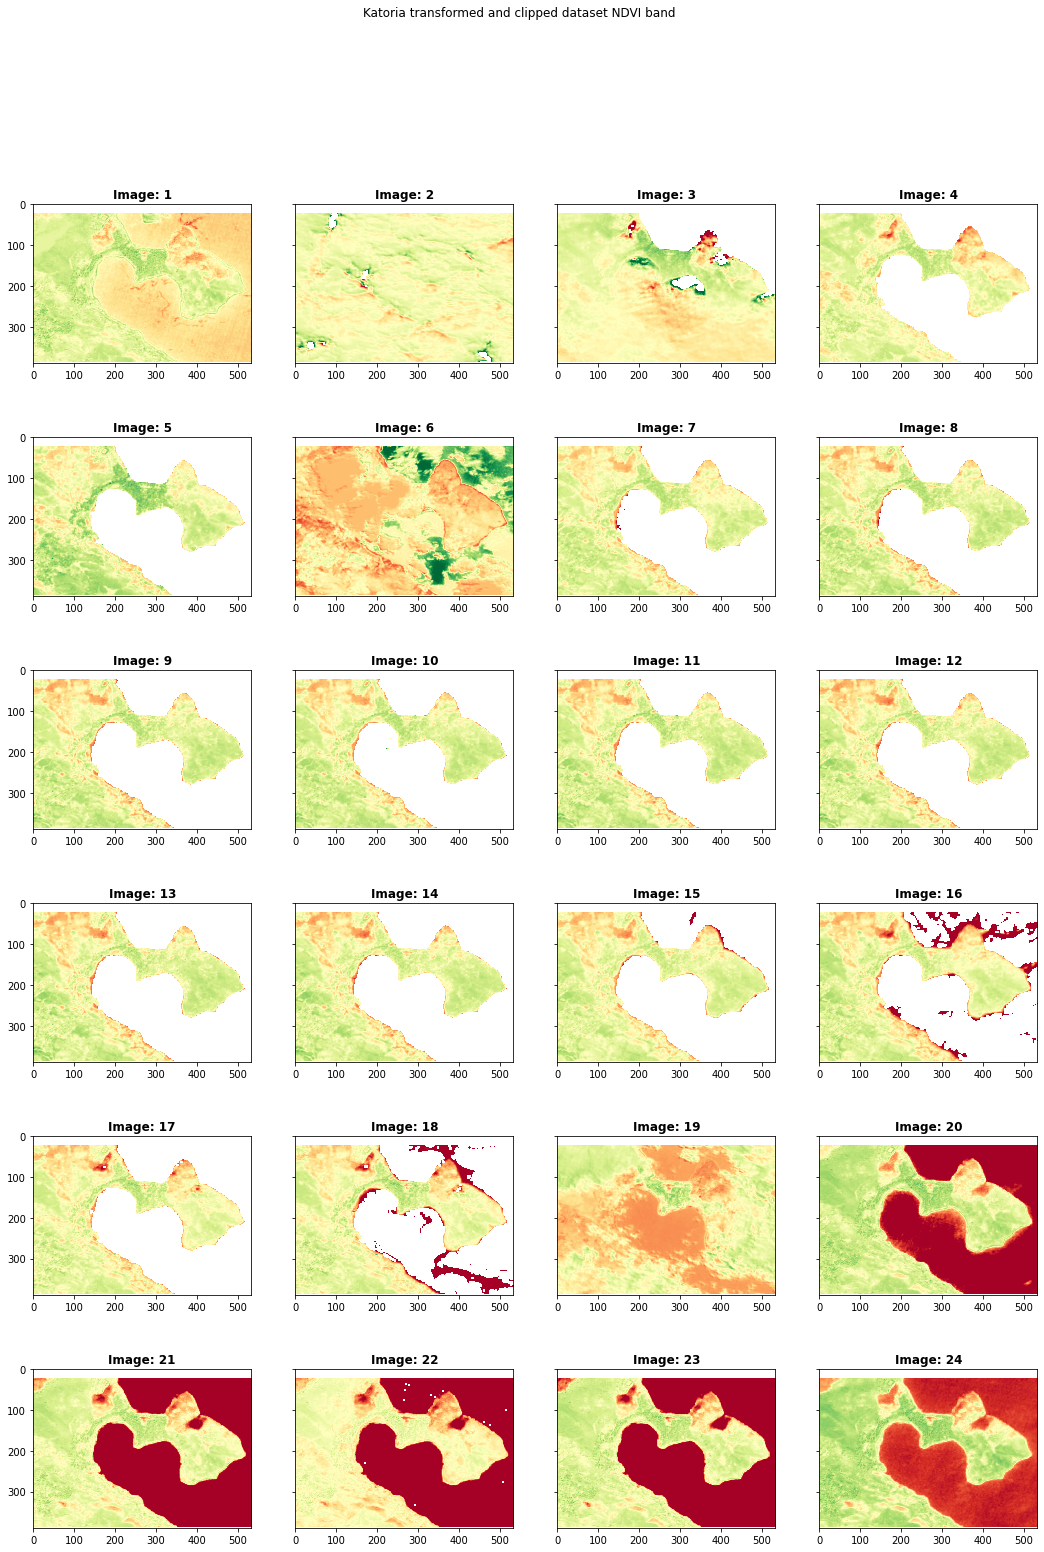
\includegraphics[width=13cm]{figures/q2_2_ROI_clipped_ndvi_for_all_dates_images.png}
    \caption{Kastoria ROI, Clipped dataset image collection, band: NDVI}
    \label{fig:Kastoria ROI, Clipped dataset image collection, band: NDVI}
\end{figure}
\FloatBarrier %fix position of image to its own subsection, not the next

The previous NDVI band plot for each date was presented in a red-yellow-green color map.

Also, the average NDVI index value for each pixel over the 24 images has been calculated and summarized in a single plot that follows. The minimum pixel ndvi value in this image that contains average ndvi pixel values is $-0.635$ whereas the maximum value is $0.641$. 

\begin{figure}[h]
    \centering
    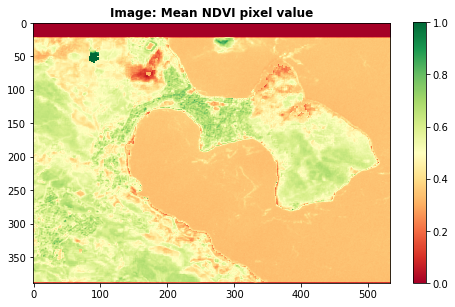
\includegraphics[width=7cm]{figures/q2_3_ROI_clipped_avg_ndvi_pixels.png}
    \caption{Kastoria ROI, average NDVI pixel value}
    \label{fig:Kastoria ROI, average NDVI pixel value}
\end{figure}
\FloatBarrier %fix position of image to its own subsection, not the next

\subsection{Question 2.4}
Following on with our NDVI band analysis, we present a graph with the progress of the NDVI index in time for the ROI For this task we will calculate the mean value of all pixels of the NDVI band for each image/date and then plot the resulting time series.

\begin{figure}[h]
    \centering
    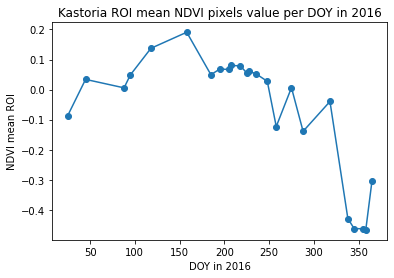
\includegraphics[width=7cm]{figures/q2_4_ROI_clipped_mean_ndvi_timeseries.png}
    \caption{Kastoria ROI, average NDVI per DOY timeseries}
    \label{fig:Kastoria ROI, average NDVI per DOY timeseries}
\end{figure}
\FloatBarrier %fix position of image to its own subsection, not the next

We observe that the highest mean NDVI pixels value is found on the 158th day of 2016 (2016-06-06), right in the summer which is what we would expect. On the contrary, we observe lower values for winter months towards the end of year 2016 and at the beginning of it. Also, given that the ROI selected contains a large part of water area, the NDVI mean values are fluctuating around 0, whereas if the area was mostly land, we might have expected higher mean ndvi values.

\section{Question 3}
In this section of the assignment, we experiment with several geospatial queries and operations utilizing the geopandas library for vector data and we subsequently create static maps. Also, we do present graphs with the time evolution of meteorological variables.

\subsection{Question 3.1}
Firstly, we download vector data from \href{https://geodata.gov.gr}{https://geodata.gov.gr}. Geodata offers vector data for a range of topics eg. points of the country's airports, public transport stations and playgrounds among others. The way we download the data is by connecting to the WFS service geodata offers through OWSLib library. We can then inspect the available vector data to retrieve from the service.

We inspect first the airports of Greece. Below is a table of the 74 airports fetched from geodata Web Feature Service (WFS).

\begin{figure}[h]
    \centering
    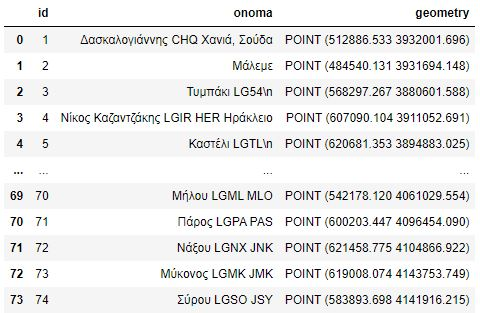
\includegraphics[width=10cm]{figures/q3_1_airports_df.JPG}
    \caption{Greece, airports table}
    \label{fig:Greece, airports table}
\end{figure}
\FloatBarrier %fix position of image to its own subsection, not the next

Prior to placing markers on a map of Greece, eg a marker for each airport, we need to find a raster RGB image of Greece. Towards this purpose we can use a Web Map Service (WMS) to download a raster RGB image that contains Greece (eg European raster image) and then select a bounding box for Greece. We selected \href{https://www.geoseer.net/rl.php?ql=78ea2e14b2fdd525&p=1&q=landsat\%20150\%20Europe#}{this} WMS service for Europe that was found through \href{https://www.geoseer.net}{Geoseer} spatial data search engine. Upon making a getmap request to the WMS service, we get a EPSG:4326 crs image of Greece, where we set the bounding box based on the coordinates found \href{https://gist.github.com/graydon/11198540}{here}. The image is saved as a geotiff and we present it below (in RGB):

\begin{figure}[h]
    \centering
    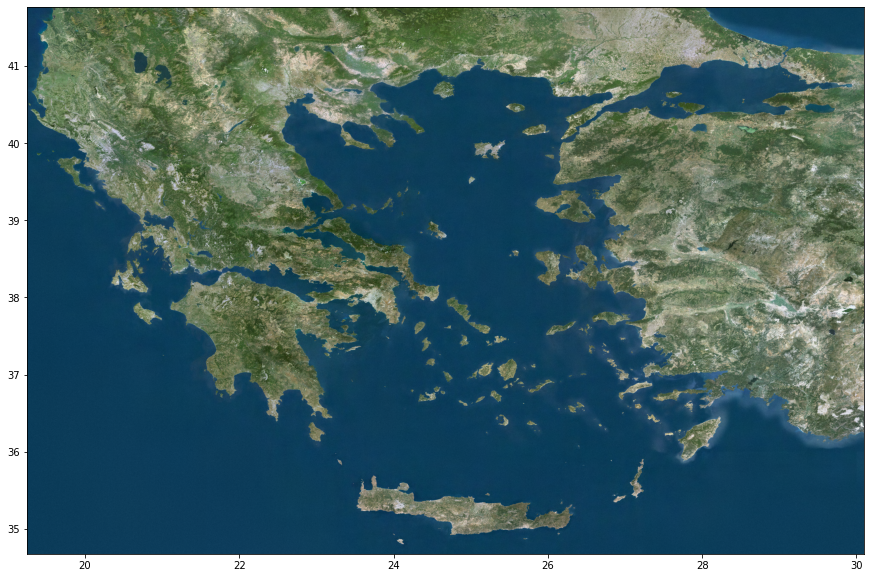
\includegraphics[width=10cm]{figures/q3_1_Greece_RGB_map.png}
    \caption{Greece, RGB raster basemap}
    \label{fig:Greece, RGB raster basemap}
\end{figure}
\FloatBarrier %fix position of image to its own subsection, not the next

Then, to add on top of the map any vector geometries, we need to first convert their crs to the same crs as the raster, which is EPSG:4326. The first layer we add on the map is that of airports, where we denote each airport's location with a black marker.

\begin{figure}[h]
    \centering
    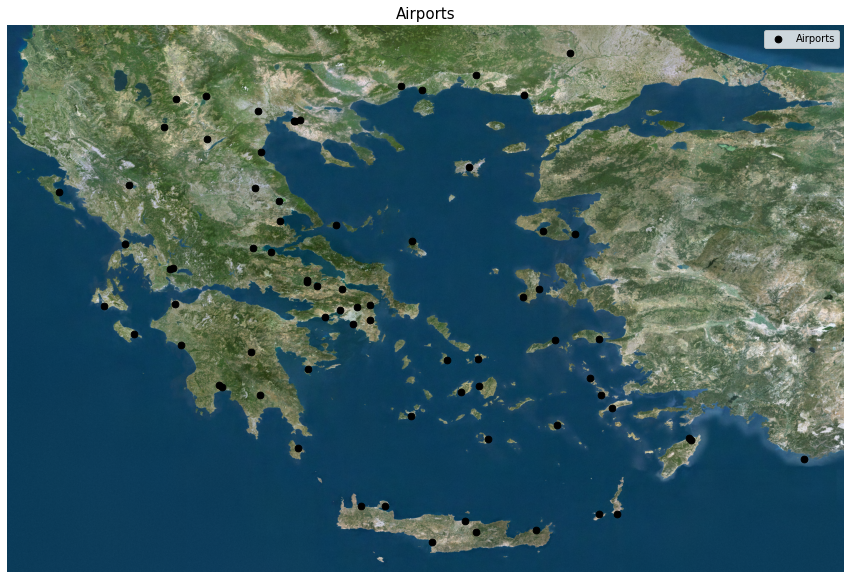
\includegraphics[width=10cm]{figures/q3_1_Greece_RGB_map_airports.png}
    \caption{Greece, RGB raster & airports}
    \label{fig:Greece, RGB raster & airports}
\end{figure}
\FloatBarrier %fix position of image to its own subsection, not the next

We can stack layers on a single raster image, for instance we next present a map with two layers, the previous one with the airports of Greece and another one containing the hydragraphic network of the country.

\begin{figure}[h]
    \centering
    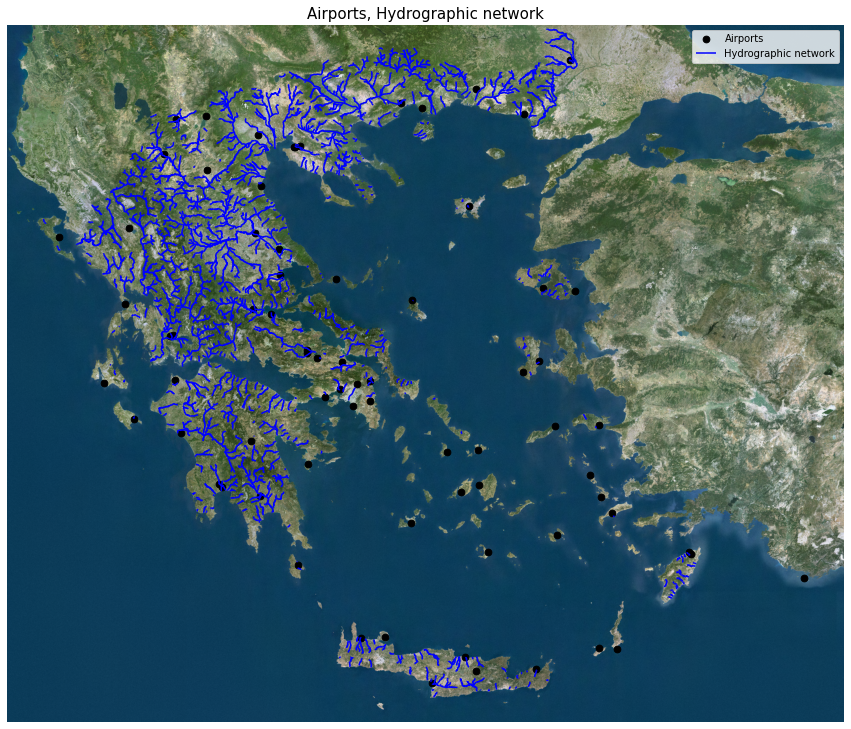
\includegraphics[width=8.1cm]{figures/q3_1_Greece_RGB_map_airports_hydrographic.png}
    \caption{Greece, RGB raster & airports & hydrographic network}
    \label{fig:Greece, RGB raster & airports & hydrographic network}
\end{figure}
\FloatBarrier %fix position of image to its own subsection, not the next

On top of the above, we create another map by combining the raster image with the layer containing Greece's counties below. We can then distinguish the borders of different counties in Greece. 

\begin{figure}[h]
    \centering
    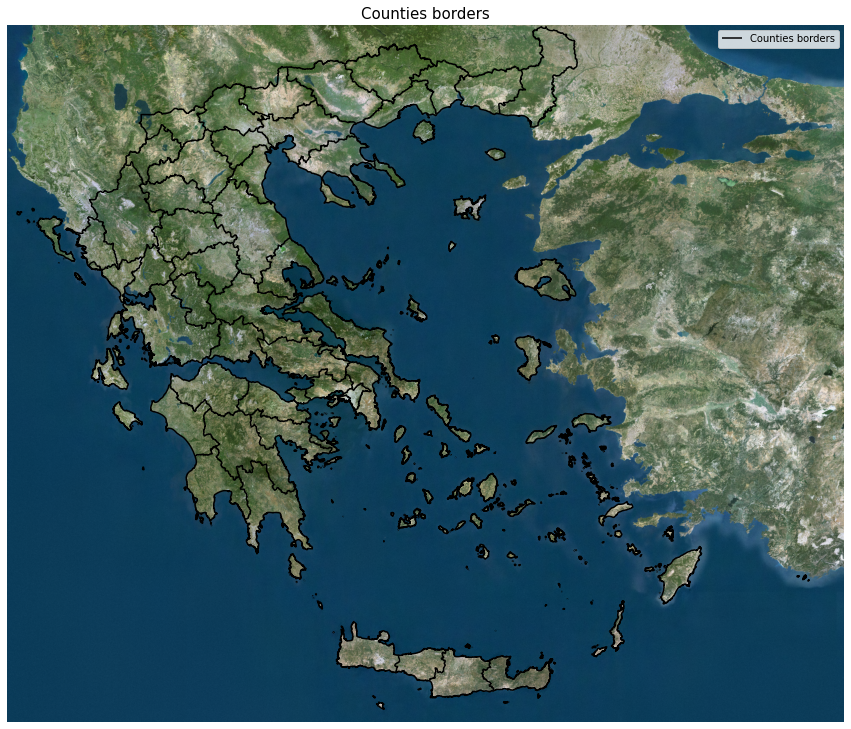
\includegraphics[width=8.1cm]{figures/q3_1_Greece_RGB_map_counties.png}
    \caption{Greece, RGB raster & counties' borders}
    \label{fig:Greece, RGB raster & counties' borders}
\end{figure}
\FloatBarrier %fix position of image to its own subsection, not the next

\subsection{Question 3.2}
Next, we implement spatial queries with the geopandas library. The first query we implemented concerns finding of the top 10 regions in Greece with the highest energy demand levels with regards to household heating based on 2015 \href{https://geodata.gov.gr/en/dataset/zetese-energeias-gia-thermanse-apo-noikokuria/resource/b53ed012-b842-47e7-9eee-851624b1a014}{data}.  

\begin{figure}[h]
    \centering
    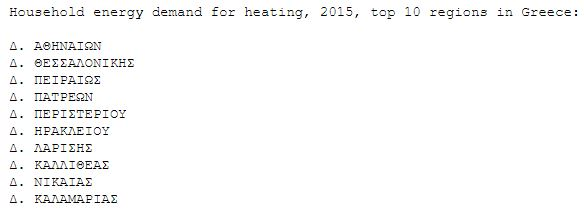
\includegraphics[width=12cm]{figures/q3_2_top_heating_table.JPG}
    \caption{Greece, Top 10 regions in heating energy demand 2015 table}
    \label{fig:Greece, Top 10 regions in heating energy demand 2015 table}
\end{figure}
\FloatBarrier %fix position of image to its own subsection, not the next

\begin{figure}[h]
    \centering
    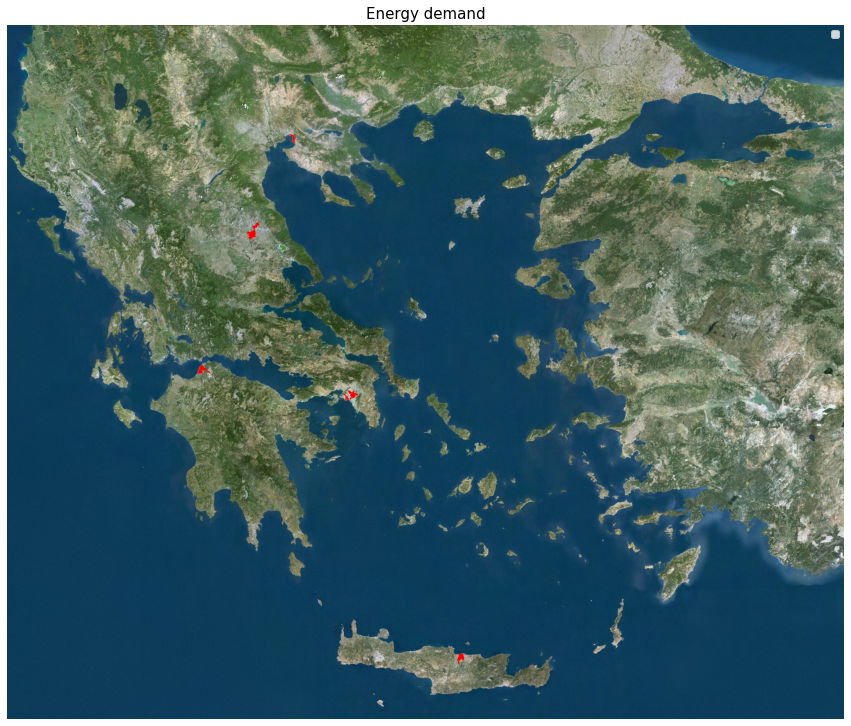
\includegraphics[width=11cm]{figures/q3_2_top_heating_map.png}
    \caption{Greece, RGB raster & top 10 regions in heating energy demand 2015}
    \label{fig:Greece, RGB raster & top 10 regions in heating energy demand 2015}
\end{figure}
\FloatBarrier %fix position of image to its own subsection, not the next

Up next, we calculate the municipalities of Greece that contain at least one airport. Below, we present the top 5 municipalities in terms of the number of airports as well as a map with the municipalities that contain airports in their territories.

\begin{figure}[h]
    \centering
    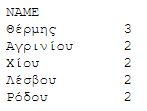
\includegraphics[width=3cm]{figures/q3_2_most_airports_table.JPG}
    \caption{Greece, Top 5 municipalities having most airports in their territories}
    \label{fig:Greece, Top 5 municipalities having most airports in their territories}
\end{figure}
\FloatBarrier %fix position of image to its own subsection, not the next

\begin{figure}[h]
    \centering
    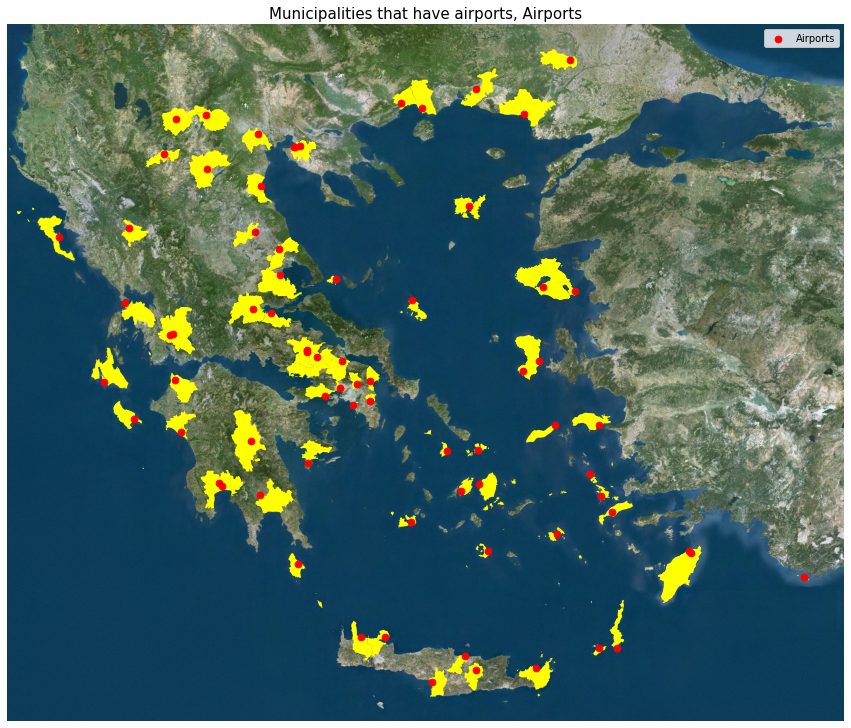
\includegraphics[width=11cm]{figures/q3_2_airports_and_municipalities_map.png}
    \caption{Greece, RGB raster & municipalities containing airports}
    \label{fig:Greece, RGB raster & municipalities containing airports}
\end{figure}
\FloatBarrier %fix position of image to its own subsection, not the next

For the next query, we further narrow down the raster image to present Athens in the raster image as a basemap.

\begin{figure}[h]
    \centering
    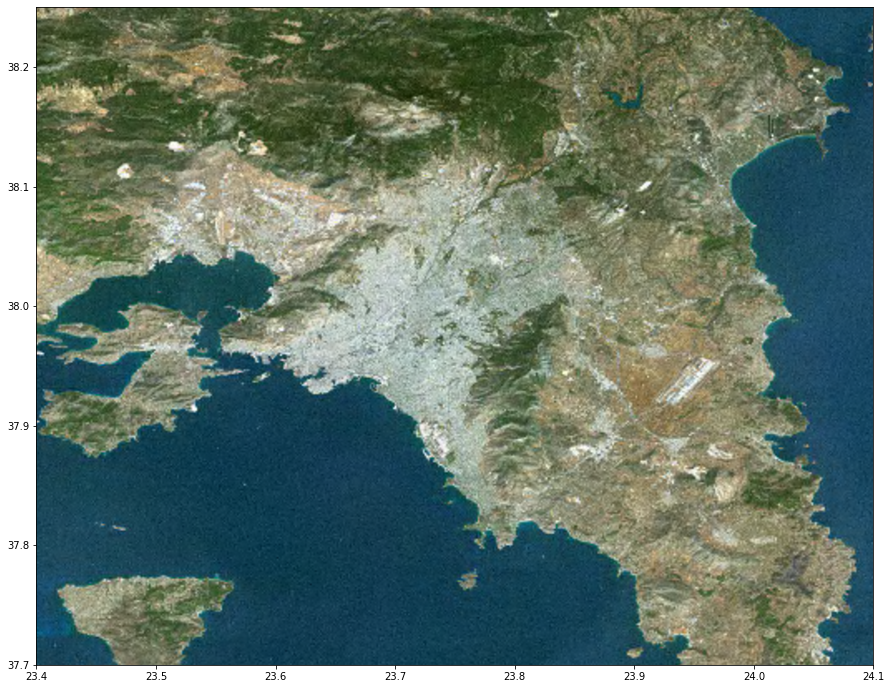
\includegraphics[width=11cm]{figures/q3_2_athens_map.png}
    \caption{Athens, RGB raster}
    \label{fig:Athens, RGB raster}
\end{figure}
\FloatBarrier %fix position of image to its own subsection, not the next

A first layer we can add is one containing markers for the public transport's stations in Athens. There is a total of $7935$ stations in Athens.

\begin{figure}[h]
    \centering
    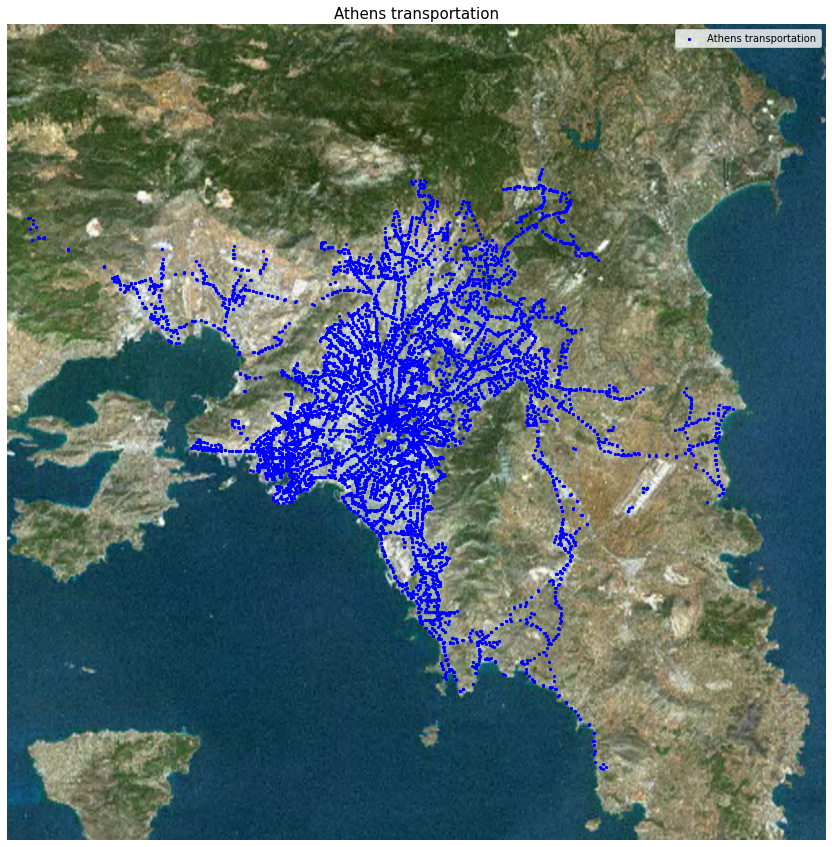
\includegraphics[width=11cm]{figures/q3_2_athens_oasa.png}
    \caption{Athens, RGB raster & public transport stations}
    \label{fig:Athens, RGB raster & public transport stations}
\end{figure}
\FloatBarrier %fix position of image to its own subsection, not the next

We now distinguish the means of transport (ie bus-trolley, suburban railway, metro-isap, metro-suburban railway, tram) that the stations benefit and present them as different layers on the same raster basemap of Athens. It becomes obvious from the plot, that the majority of stations are bus-trolley stations.

\begin{figure}[h]
    \centering
    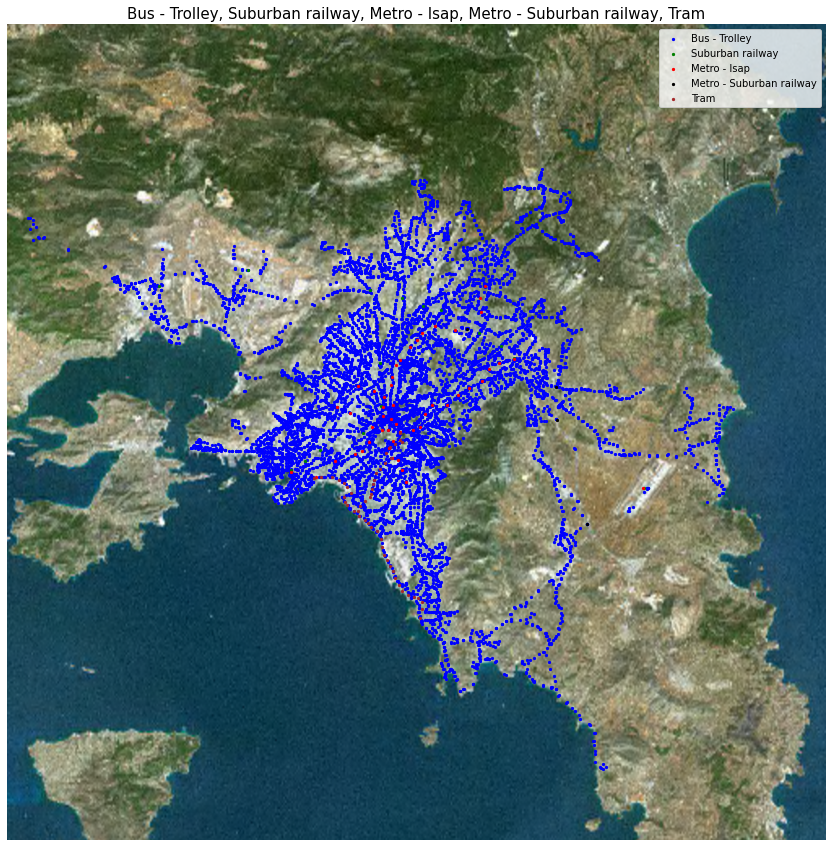
\includegraphics[width=11cm]{figures/q3_2_athens_oasa_split.png}
    \caption{Athens, RGB raster & public transport stations by means of transport}
    \label{fig:Athens, RGB raster & public transport stations by means of transport}
\end{figure}
\FloatBarrier %fix position of image to its own subsection, not the next

\subsection{Question 3.3}
In this section, we now load Corine Land Cover (CLC) 2018 data for a selected ROI from a WFS service. As described by \href{https://land.copernicus.eu/news/corine-land-cover-now-updated-for-the-2018-reference-year}{Copernicus}, it is one of the most widely used products from the Copernicus Land Monitoring Service that consists of an inventory of land cover in 44 classes.

We now select Belgium as the region of interest (ROI). Searching in \href{https://www.geoseer.net/}{Geoseer}, we came up with the \href{https://wms.ngi.be/inspire23/landcover/wfs}{wfs service} to use for retrieving the CLC 2018 data. Within the data downloaded, the land cover class is given under \emph{lcclass} variable as a 3-digit integer and there are 44 discrete numbers for a matching number of classes. A mapping of the 3-digit classes encoding to their label/usage is provided \href{https://collections.sentinel-hub.com/corine-land-cover/readme.html}{here}.

Also, we located a \href{https://wms.ngi.be/inspire23/landcover/ows?SERVICE=WMS&}{wms service} again through \href{https://www.geoseer.net/}{Geoseer's} search in order to retrieve Belgium's raster landcover image.

In order to convert the 3-digit numbers of the vector data, we download an \emph{xlsx} \href{https://www.eea.europa.eu/data-and-maps/data/corine-land-cover-2000-clc2000-100-m-version-9-2007/corine-land-cover-2000-classes-and-rgb-color-codes/clc2000legend.xls}{file} that contains mappings of the 3-digit codes to the string labels with the land cover usage. From this exact same file we also extract the RGB hex code for each code. This is the RGB color that is assigned to each pixel based on its 3-digit code characterization of its land usage.

As a next step, the European raster image is clipped in order to retrieve an RGB raster basemap of Belgium.

\begin{figure}[h]
    \centering
    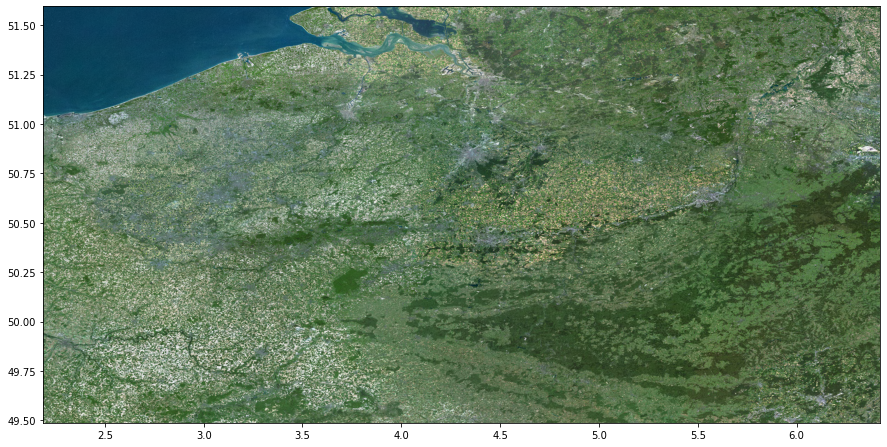
\includegraphics[height=6cm]{figures/q3_3_belgium_map.png}
    \caption{Belgium, RGB raster}
    \label{fig:Belgium, RGB raster}
\end{figure}
\FloatBarrier %fix position of image to its own subsection, not the next

Then, we add the wms CLC layer on top and we receive the following image.

\begin{figure}[h]
    \centering
    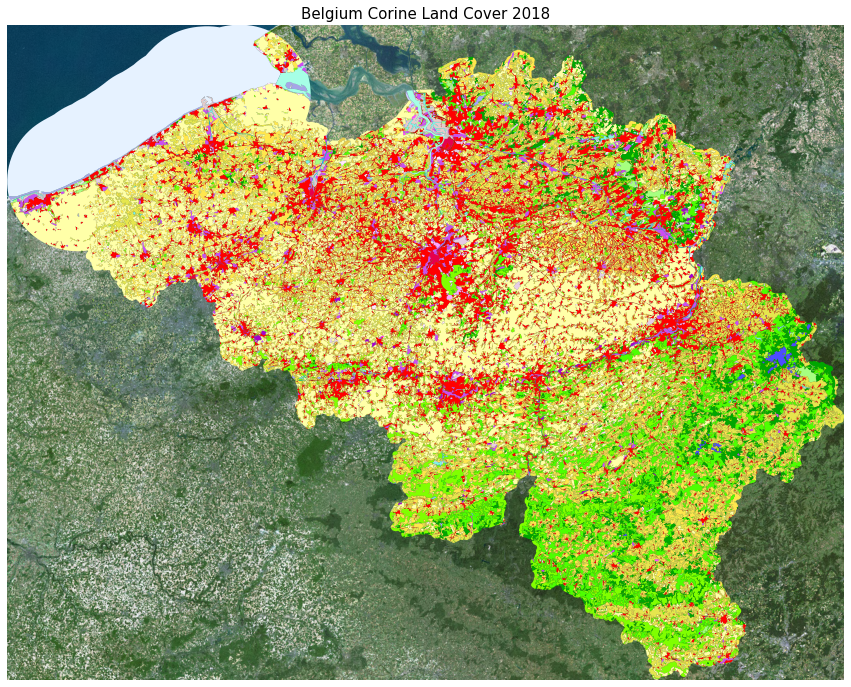
\includegraphics[width=11cm]{figures/q3_3_belgium_map_and_clc2018.png}
    \caption{Belgium, RGB raster & CLC 2018}
    \label{fig:Belgium, RGB raster & CLC 2018}
\end{figure}
\FloatBarrier %fix position of image to its own subsection, not the next

\subsection{Question 3.4}
Up next is the retrieval and presentation of meteorological time series data for an area of interest. We now select a point in the center of Ghent, one of the major cities of Belgium (north Belgium). We select the exact point and coordinates using \href{https://geojson.io/}{geojson} and download the generated shapefile. In the image below, we can see the selected point in geojson's user web interface.

\begin{figure}[h]
    \centering
    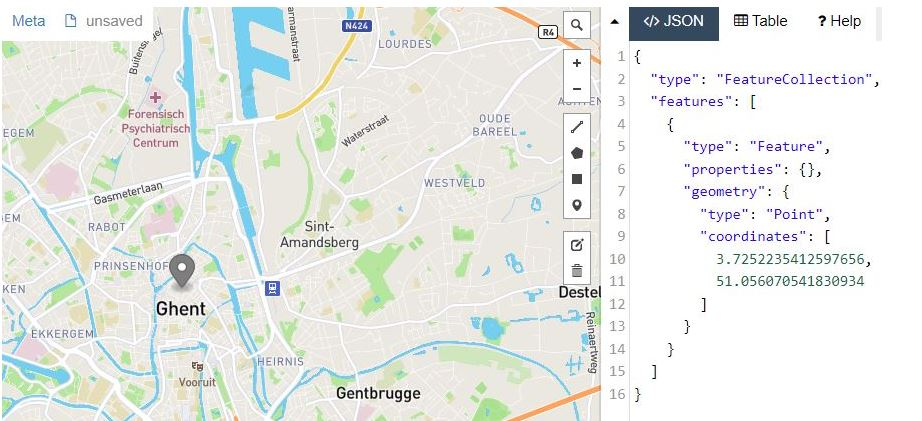
\includegraphics[width=11cm]{figures/q3_4_ghent_geojson_point.JPG}
    \caption{Ghent, geojson ROI}
    \label{fig:Ghent, geojson ROI}
\end{figure}
\FloatBarrier %fix position of image to its own subsection, not the next

We then download meteorological data from \href{https://power.larc.nasa.gov/data-access-viewer/}{NASA}  for the ROI (point/marker in Ghent) and for the period between 01-01-2020 - 01-01-2022 and more specifically the following data:

\begin{itemize}
    \item Temperature at 2 Meters (C)
    \item Relative Humidity at 2 Meters (\%)
    \item Precipitation (Corrected, mm/day)
    \item Wind Speed at 10 Meters (m/s)
\end{itemize}

We then proceed to generating the plot of the temperature at 2 meters for the point of interest over time.

\begin{figure}[h]
    \centering
    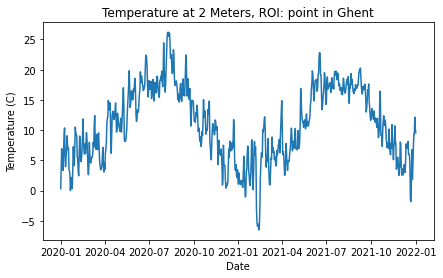
\includegraphics[width=11cm]{figures/q3_4_temperature.png}
    \caption{Ghent, ROI temperature at 2 meters timeseries}
    \label{fig:Ghent, ROI temperature at 2 meters timeseries}
\end{figure}
\FloatBarrier %fix position of image to its own subsection, not the next

We can see there is periodicity on the temperature levels for the selected point, peaking during sumer months (July-August) as one would expect.

Next, we plot the timeseries for the wind speed at 10 meters in m/s. We can observe that windspeed, unlike temperature, exhibits very quick changes in its value within short time periods. However, no clear pattern can be detected apart from the observation that during some periods smaller peaks are detected.

\begin{figure}[h]
    \centering
    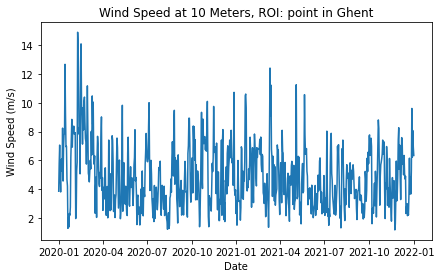
\includegraphics[width=11cm]{figures/q3_4_wind_speed.png}
    \caption{Ghent, ROI wind speed at 10 meters timeseries}
    \label{fig:Ghent, ROI wind speed at 10 meters timeseries}
\end{figure}
\FloatBarrier %fix position of image to its own subsection, not the next

Below, we additionally plot the timeseries for the relative humidity percentage for the ROI. Here, we can see there is some periodicity on the humidity levels where the high peaks are observed during winter time and the low peaks in summer time.

\begin{figure}[h]
    \centering
    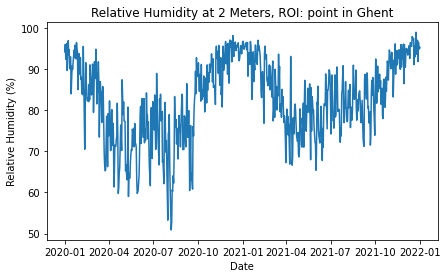
\includegraphics[width=11cm]{figures/q3_4_relative_humidity.png}
    \caption{Ghent, ROI relative humidity at 2 meters timeseries}
    \label{fig:Ghent, ROI relative humidity at 2 meters timeseries}
\end{figure}
\FloatBarrier %fix position of image to its own subsection, not the next

Lastly, we present the plot for the corrected precipitation (mm/day) timeseries, where we can see that there is a continuous of days with relatively high precipitation values during winter months, however this is not the case in spring/summer months.

\begin{figure}[h]
    \centering
    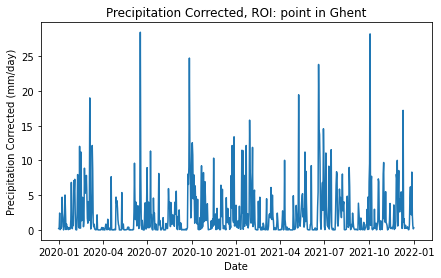
\includegraphics[width=11cm]{figures/q3_4_relative_precipitation.png}
    \caption{Ghent, ROI precipitation (corrected) timeseries}
    \label{fig:Ghent, ROI precipitation (corrected) timeseries}
\end{figure}
\FloatBarrier %fix position of image to its own subsection, not the next

\section{Question 4}
In this final part of the assignment, we present an interactive map of Greece using folium and combining raster and vector data of our choice.

We select to present a raster image as a layer on the map on top of a street map basemap. The raster image is a European one and centered to Greece. Then, we add vector data as layers too. The interactive map is available also in html format as a standalone file apart from the \emph{ipynb} file. The file can be viewed on any browser and users can interact with the map. 


All the layers presented on the map are listed below:

\begin{enumerate}
  \item Raster:
  \begin{enumerate}
      \item european raster image centered to Greece
  \end{enumerate}
  \item Vector:
  \begin{enumerate}
      \item Markers:
      \begin{enumerate}
          \item Airports
          \item National Parks average centroids
          \item Lakes average centroids
          \item Wifi public spots
          \item Beaches awarded with blue flag 
          \item Dams
      \end{enumerate}
      \item Polygons:
      \begin{enumerate}
          \item National Parks
          \item Lakes
      \end{enumerate}
  \end{enumerate}
\end{enumerate}

\begin{figure}[h]
    \centering
    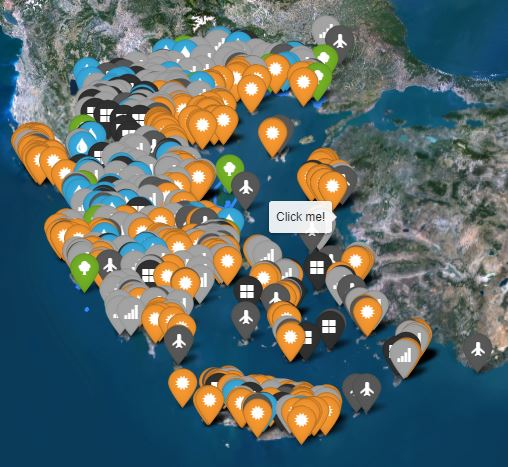
\includegraphics[width=11cm]{figures/q4_map_snippet.JPG}
    \caption{Greece, interactive map snippet}
    \label{fig:Greece, interactive map snippet}
\end{figure}
\FloatBarrier %fix position of image to its own subsection, not the next

The markers on the map are straightforward to implement, since the vector data such as the airports contain Point geometries that upon being converted to the right crs can be easily added to a Feature Group (eg airports feature group) and then the feature group is added as a layer to the map. 

However, for polygons such as national parks and lakes, there are several entries in the relevant geopandas dataframe containing the vector data for the same item (eg. several rows in the dataframe for a single national park). This means that taking the centroids of the polygons and adding them to the map would end up in several markers for each national park. In order to add a single marker for those instead, we then proceed to calculating the centroids of the polygon geometries for each entry and then aggregate the centroids for each national park and lake by taking the average coordinate of those centroids. This results in two layers for national parks and lakes, one for the polygons of the parks and lakes, and another with those centroids denoting the center of each lake and park. 

\begin{thebibliography}{9}
\bibitem{OWSLib}
OWSLib \url{https://www.osgeo.org/projects/owslib}
\bibitem{rasterio}
rasterio \url{https://rasterio.readthedocs.io/en/latest/}
\bibitem{geopandas}
geopandas \url{https://geopandas.org/}
\bibitem{folium}
folium \url{https://python-visualization.github.io/folium/}
\bibitem{leafmap}
leafmap \url{https://leafmap.org/}
\bibitem{fiona}
fiona \url{https://fiona.readthedocs.io/}
\end{thebibliography} %this tex file contains main body of our document

\end{document}







